\problemname{Pipe Rotation}

\noindent The four ninja turtles: Leonardo, Donatello, Michelangelo, and Raphael are seeking a new home in Manhattan, New York City. The turtles don't like sudden dead-ends in their home. Fortunately, the government recently installed a new sewage system where pipes can be rotated! The turtles needs your help finding a suitable home, so they're willing to provide you a grid of the current layout of the sewage system.\\

The grid consists of $N$ rows and $M$ columns. The cell $G_{i,j}$ will consist of one of four pipes, encoded as a letter between ``\texttt{A}" and ``\texttt{D}". These pipes can be rotated by any multiple of $90$ degrees:\\

\noindent
\begin{minipage}{0.25\textwidth}
  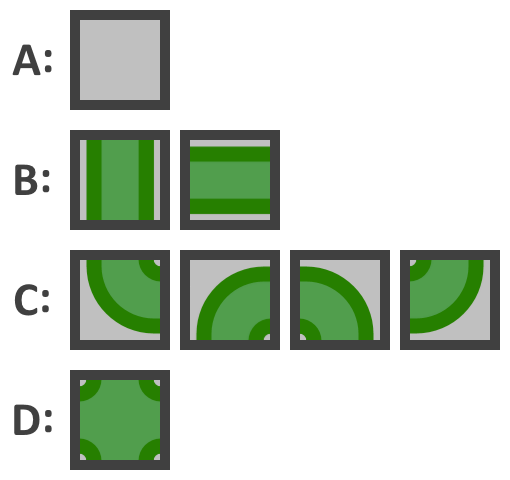
\includegraphics[width=0.95\textwidth]{pipe_rotation_1.png}
\end{minipage}
\begin{minipage}{0.75\textwidth}
  \begin{itemize}
    \item (\texttt{A}) Nothing
    \item (\texttt{B}) Straight pipe (pipes leaving through two opposite edges)
    \item (\texttt{C}) Elbow-shaped pipe (pipes leaving through two adjacent edges)
    \item (\texttt{D}) Four-way pipe (pipes leaving through all four edges)
  \end{itemize}
\end{minipage}
\vspace{10pt}

Determine whether it's possible to rotate the cells such that the pipes all line up with one another. In particular, for each edge shared by a pair of adjacent cells, there must either be a pipe on both sides of that edge, or on neither side. And for each each of the $2 \cdot (N + M)$ outer edges of the grid, there must be no pipe leaving through that edge. Below are examples:

\begin{figure}[h]
  \centering
  \begin{minipage}[t]{0.3\textwidth}\centering
      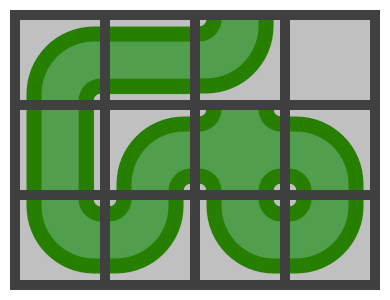
\includegraphics[width=0.95\textwidth]{pipe_rotation_2}
      Fig 1. Invalid example,\\ two sudden dead-ends.
  \end{minipage}
  \hspace{30pt}
  \begin{minipage}[t]{0.3\textwidth}\centering
      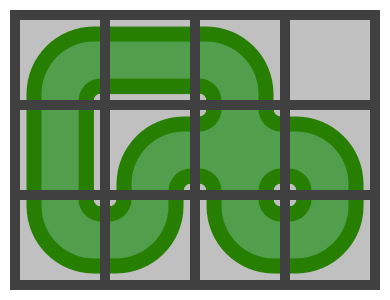
\includegraphics[width=0.95\textwidth]{pipe_rotation_3}
      Fig 2. Valid example,\\ no sudden dead-ends.
  \end{minipage}
\end{figure}

\section*{Input}
The first line of input consists of two space-separated integers, $N$ and $M$ ($1 \leq N, M \leq 100$).\\
$N$ lines follow, the $i$th of which consists of $M$ characters $G_{i,1}, G_{i,2}, G_{i,j}, \dots, G_{i,M}$ and $G_{i,j} \in \{A,B,C,D\}$ (for $i = 1..N$).

\section*{Output}
Print, on a single line, a single string, either ``\texttt{Possible}" if it's possible to produce a valid configuration of pipes, or ``\texttt{Impossible}" otherwise.\\
